\chapter{Trabajos Relacionados}
\label{chap:cha3}

En este capítulo está destinado a explicar el estado del arte de las investigaciones relacionadas a la propuesta de tesis.
Este capítulo debe contener un buen número de referencias y no debe exceder tres páginas de texto. Para esto se puede tomar como ejemplo la forma de hacer una revisión bibliográfica en un artículo científico.

Este es un ejemplo de como realizar una referencia implícita \citep{Yasmin2015} y unas referencias explícitas \citet{Furini2008, Avila2011}.


La figura \ref{fig:Pipeline2} es un ejemplo de como insertar y referenciar una imagen.
Este es un ejemplo de enumerado.


\begin{enumerate*}
\item[(a)] Primer item
\item[(b)] Segundo item
\item[(c)] Tercer item
\end{enumerate*}.


Ejemplo de como insertar imagenes:
% Insertando imagen.
  \begin{figure}
  \centering
  \subfloat[]{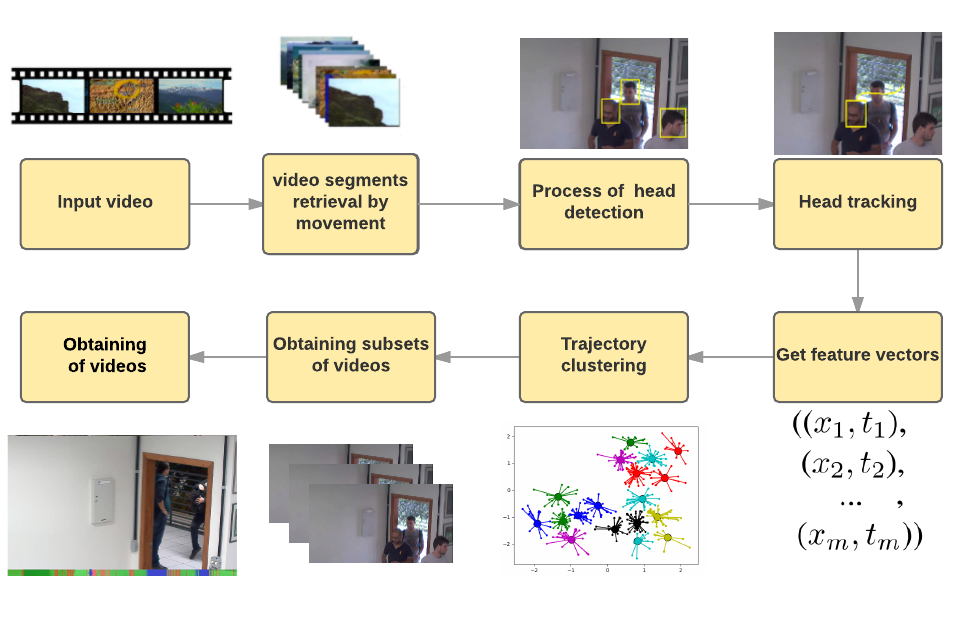
\includegraphics[width=6in]{graficos/pipeline2.png}}
  \caption[Imagen ilustrativa.]
  {Imagen ilustrativa. Imagen ilustrativa de como se puede insertar una imagen con latex.}
  \label{fig:Pipeline2}
  \end{figure}
% Fin de insertando de imagen






